\documentclass{kybernetika}
%the class kybernetika includes these packages:
% graphicx, amssymb, amsmath

%DEBUG ONLY
\usepackage{layouts}

%--------------------------------------------------------------------------------------------------
% used environment for theorems:

\newtheorem{theorem}{Theorem}[section]
\newtheorem{lemma}[theorem]{Lemma}
\newtheorem{proposition}[theorem]{Proposition}
\newtheorem{corollary}[theorem]{Corollary}
\newtheorem{remark}[theorem]{Remark}
\newtheorem{fact}[theorem]{Fact}
\newtheorem{example}[theorem]{Example}
\newtheorem{definition}[theorem]{Definition}
\newtheorem{observation}[theorem]{Observation}

\begin{document}

%==================================================================================================
% TITLE PAGE 
%==================================================================================================
\pagestyle{myheadings}
\title{Application of Long Short Term Memory neural networks for GPS satellite clock 
bias prediction}

\author{Piotr Gny\'{s}, Pawe\l{} Przestrzelski}

\contact{Piotr}{Gny\'{s}}
{Department of Computer Science,  Polish-Japanese Academy of Information Technology,
Koszykowa 86 Street, 02-008 Warsaw}{pgnys@pjwstk.edu.pl}

\contact{Pawe\l{}}{Przestrzelski}
{Department of Computer Science,  Polish-Japanese Academy of Information Technology,
Koszykowa 86 Street, 02-008 Warsaw}{pprzestrzelski@pjwstk.edu.pl}

\markboth{Piotr Gny\'{s}, Pawe\l{} Przestrzelski}{LSTM networks for GPS clock bias prediction}

\maketitle

\begin{abstract}
In this article the results of an application of Long Short Term Memory neural networks for
clock bias will be presented and compared against current state of the art in real-time
GPS clock bias prediction. Presented approach is intended to better quality of localization
for marine robots that operate autonomously for long periods of time away from convenient  
internet uplink.
textwidth in cm: \printinunitsof{cm}\prntlen{\textwidth}
\end{abstract}

\keywords{LSTM, Long Short Term Memory, Neural Networks, GPS, Navigation, Time series prediction}

\classification{68T05, 68T10, 68T40}


%==================================================================================================
\section{Introduction}
Research presented in this paper is part of a larger project that aims at developing a long
term autonomous marine robotics systems. However as Global Positioning System (GPS) is used
in many application elements specific to one that was intended when working on algorithm will
be omitted with exception of MOTIVATIONS section.

%--------------------------------------------------------------------------------------------------
\subsection{Motivation}
In recent years there was a rise in popularity of autonomous platforms. Examples include, but
are not limited to, Tesla self driving cars, autonomous container ships or robotic defence 
systems. All those applications have one thing in common, they require a precise navigation 
capabilities that will allow them to move without damaging themselves or their environments. 
This is especially challenging in marine environment as not only there is almost no visual
reference points on open see but also because any contact with external data source is expensive
as very often only connection available is satellite uplink.
In case of large vessels, like already mentioned autonomous container ships, this is only
problem of bandwidth cost. 
However in case of small robots like gliders or sailboats that rely on low power consumption 
any localization system is limited by low computation power and high energy consumption of 
satellite communication that discourages it frequent use.
This is why an effort was made to deploy a solution that provides a on-board solution for high
quality GPS based localisation with low computational overhead.

%--------------------------------------------------------------------------------------------------
\subsection{Contribution}
In following paper a new approach for GPS clock bias prediction based on a Long Short Term Memory
neural networks is presented. For 20 out of 29 satellites that were analysed in this work 
prediction results were better than current state of the art and for 6 of them results were
significantly better. Results of presented research can be used in a offline GPS receiver as 
a alternative for IGU provided products.


%==================================================================================================
\section{Clock bias in GNSS}
Due to the nature of GNSS precision time measurement is crucial for correct localisation.
In this section more inforation about why it is so and what is current state of the art on this
topic will be presented.

%---------------------------------------------------------------------------------------------------
\subsection{Importance of clock bias in localisation}
All global satellite navigation systems (GNSS) are variant of beacon based localization
systems\cite{Blewitt1997}.Such systems require information about beacon position
and distance between localized object and beacons.
With that information it is possible to calculate position of object in same reference
frame as that of beacons.
Both of those tasks are much more difficult in GNSS due to a nature of the beacons.
Unlike in case of a stationary beacons GNSS satellites move with high speed so
their position must be calculated based on satellite ephemeris\cite{Vallado2008}.
Another problem is distance measurement which without specialised equipment must be
done with time of arrival (ToA) instead of angle of arrival (AoA) or
received signal strength (RSS) \cite{Doberstein2012}.
When measuring distance by ToA  3 properties of a signal must be known:
\begin{itemize}
\item $t_o$ : time of origination
\item $t_a$ time of arrival
\item $v$ velocity
\end{itemize}
In case of GNSS system signal is a electromagnetic wave therefore its speed is equal
to speed of light $c\approx 3*10^{9} \frac{m}{s}$. Time of arrival is recoded when
data frame wavefront reaches receiver, this means that receiver time is used.
Origination time is recorded on satellite according to it local clock and
included in data frame. Thanks to that distance can be calculated by simple
equation:
\begin{equation}
  d=c*(t_a-t_o)
\end{equation}
However $t_a$ and $t_o$ are using different reference frame so for comparison
to be possible they must be transformed into a common reference frame.
This is refered to as a synchronisation of the clocks and is very important as
a desynchronisation on level of single nanosecond results in about 30 cm of
positioning error\cite{Enge2011}.
While actual calculations 

%--------------------------------------------------------------------------------------------------
\subsection{IGU products}
The most widely used source of precise clock corrections are products provided 
by International GNSS Service (IGS) \cite{IGS}.
% TODO:Fix table size so it is not wider than text
\begin{table}[ht] 
	\centering
	\caption{Variants of IGS products}
	\label{tab:igs_products}
	\begin{tabular*}{\textwidth}{*{5}{l}}
		\hline
		\hline
		Type& Accuracy& Latency& Update& Sample \\
		&&&&interval\\
		\hline
		Transmitted & 5ns & real time & -- & daily  \\
		Ultra rapid -- predicted & 3ns & real time & at 03, 09, 15, 21 UTC & 15 min  \\
		Ultra rapid -- observed & 150ps & 3-9 hours & at 03, 09, 15, 21 UTC & 15 min  \\
		Rapid & 75ps & 17-41 hours & at 17 UTC daily & 5 min \\
		Final & 75ps & 12-18 days & every Thursday & 30 s \\
		\hline
		\hline
	\end{tabular*}
\end{table}
Values shown in Table \ref{tab:igs_products} refer to satellite clock bias only,  IGS products
provide other information which full description  is available at online repositiory. 
IGS products can be easily divided into two categories:
\begin{itemize}
	\item real time consisting of transmitted and ultra rapid predicted half,
	\item high latency consisting of ultra rapid observed half as well as rapid and final products.
\end{itemize}
Solutions that have high latency are not usable in real-time navigation and as such will not be
considered in this work. Ultra-rapid observed part will be used as a source of
reference time so that if a bias prediction error is equal to zero it means that is
the same as provided by Ultra-rapid observed.
As can be seen in the Table \ref{tab:igs_products} all real-time solutions provide precision 
at a range of nanoseconds, aim of this work is to show that LSTM networks can provide 
better results than those solutions while still working at real-time response latency.

%--------------------------------------------------------------------------------------------------
\subsection{Data source}
This work focuses only on GPS satellites which are divided into five groups :
Original (II), IIA, ,IIR ,IIR-M ,IIF.
As original generation was full retired in 2007 it will not be taken into consideration, while
a single satellite from generation IIA was used in second phase of experiments it was no longer
presend in following phases as that generation was fully retired in 2019.
This results in 31 individual satellites for phases 1 and 2 and 30 for phases 3 and 4.
Almost all of them are equipped with Rubidium clock ensemble witch exception of two satellites
from generation IIF that use Cesium clocks instead.
Each satellite have an assigned space vechicle number (SVN) and pseudo random noise (PRN).
In this work a PRN will be used as a identifier as it is unique for every active satellite, 
although it can be used again after said satellite gets retired, and ranges from 1 to 32.
\begin{table}[ht] \label{table:2}
\parindent0pt
\caption{Bias prediction error in relation to regularization and dropout level}
\centering
\begin{tabular}{ l  c  c }
  \hline
  \hline
  Generation& clock typt& satellites\\  \hline
  IIA & Rb& 18\\  
  IIR & Rb& 2 11 13 14 16 19 20 21 22 23 28\\ 
  IIR-M & Rb& 5 7 12 15 17 29\\ 
  IIF & Rb& 1 3 6 9 10 25 26 27 30 32\\ 
  IIF & Cs& 8 24 \\ \hline \hline
 \end{tabular}
\end{table}
For satellites with rubidium based clock ensembles bias have a very disting constant drift
that makes data appear linear, it can be seen for satellites 01 and 08. 
On the other hand in case of cesium based clock ensembles for which constant drift is much 
smaller other sources of bias are visible, like seen for satellite 24.
There is also a single satellite for which, during observed period, constant drift was almost
not present. This was satellite 14 and while no official source of information describes this 
behaviour
\begin{figure}[ht] 
\centering
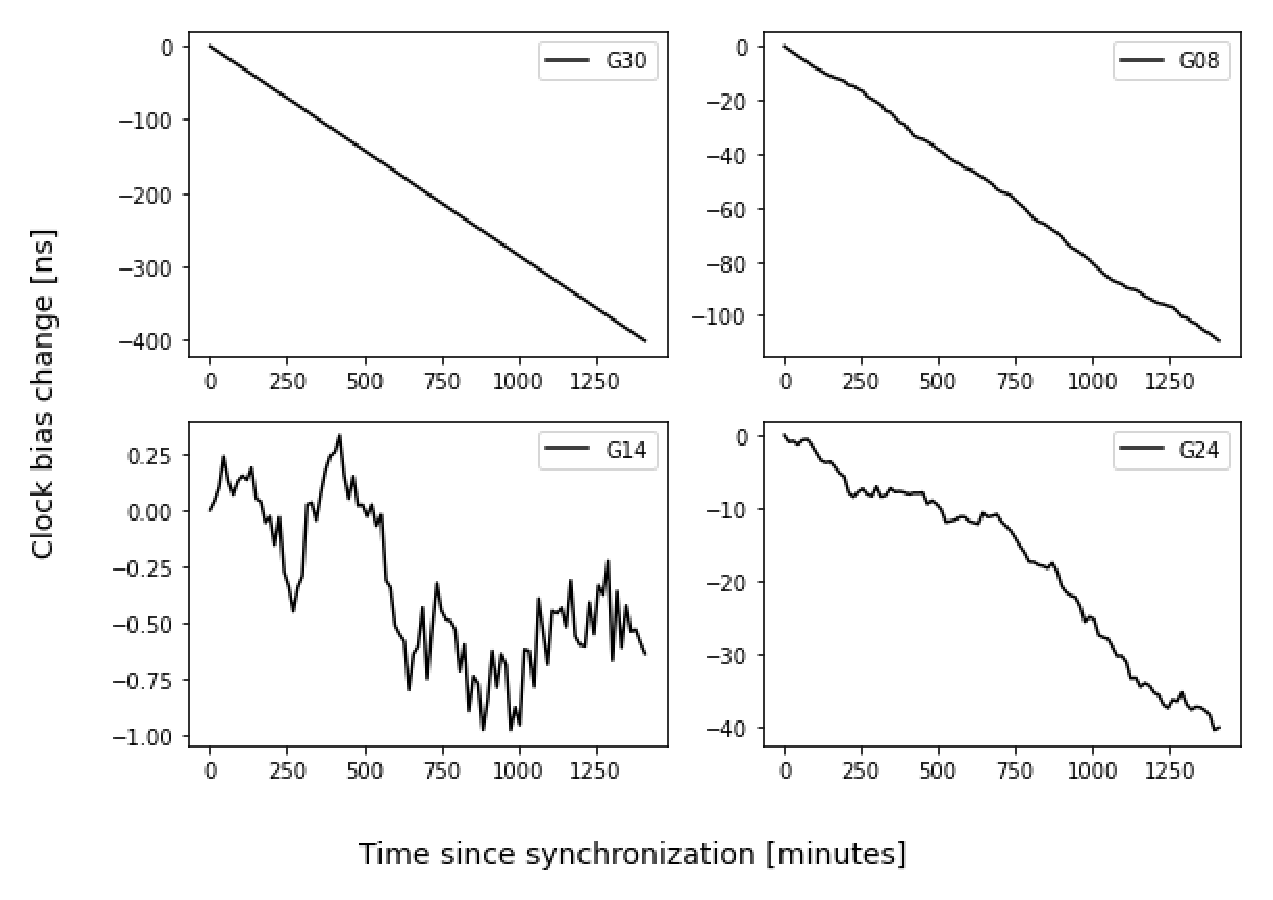
\includegraphics[width=\textwidth]{figures/bias_raw}
\caption{Raw clock bias}
\label{fig:bias_raw}
\end{figure}

%==================================================================================================
\section{Neural networks}

%--------------------------------------------------------------------------------------------------
\subsection{Overview}  
Machine learning (ML) approaches based on a artificial neural networks (ANN) are
well established as a efficient pattern detectors \cite{Abiodun2019} \cite{Miller1993}
\cite{Faraway2008} \cite{Herbrich1999} \cite{Khan2019}.
It has also been used in GNSS systems especially since advent of the deep learning
algorithms \cite{Wei2016} \cite{Kim2019} \cite{OrusPerez2019}.
One of it uses is prediction of clock bias \cite{Wang2017} \cite{Indriyatmoko2008}
which as mentioned in previous section is an essential value in positioning calculations.
Like all digital signal processing applications software neural networks operate in
discreet time and discreet amplitude domain. This is the reason why a time series clock model
was chosen. Basic model of neuron (neural layer) was created by McCullough and Pitts in 1943
\cite{McCulloch1943}. It described response of neural layer to multiple signals with
equation $y= \chi (W*x+b)$ where $y$ is response, $x$ input, $W$ weights and $b$ bias.
Algorithm for automated adjustment of weights in relation to data was proposed in 1958
While this model and its successors where inspired by a biological neuron there are much
more simplified. One of those simplification is lack of time domain in model which means
that response of a layer depends only on its current input.
This is in contrast with biological networks that are sensitive not only for signal value
but also for its change over time.

%--------------------------------------------------------------------------------------------------
\subsection{Long Short Term Memory networks}
Simple solution to problem of time independence is to concatenate response of neural layer
from previous cycle to it input $x'(t)=[x(t)|y(t-1)]$.
Such solution results in signal propagating trough time and influencing responses of future cycles,
if this is only modification to feed forward model such layer is called simple recurrent
unit (SRU).
While this solution makes model time aware it have its own problems, mainly a signal vanishing
issue. Since the input signal from cycle $n$ have direct influence only on a response of this
cycle and for each subsequent cycles it is only trough feedback loop. Influence of input $n$ on
response of cycle $n+k$ grows inverse proportional to $k$.
This means that in this model only those regularities that appear over short time periods can
be detected.
Making weights on feedback bigger will not eliminate problem and instead replace it with signal
explosion that causes response to reach maximum value if a strong signal appeared on input at
least once.
One of possible solutions to this issue is addition of long term memory which will regulate
forward and loopback path influence on neuron response, such solution is used in long short
term memory (LSTM) networks \cite{Hochreiter1997}.
\begin{figure}[ht] 
\centering
	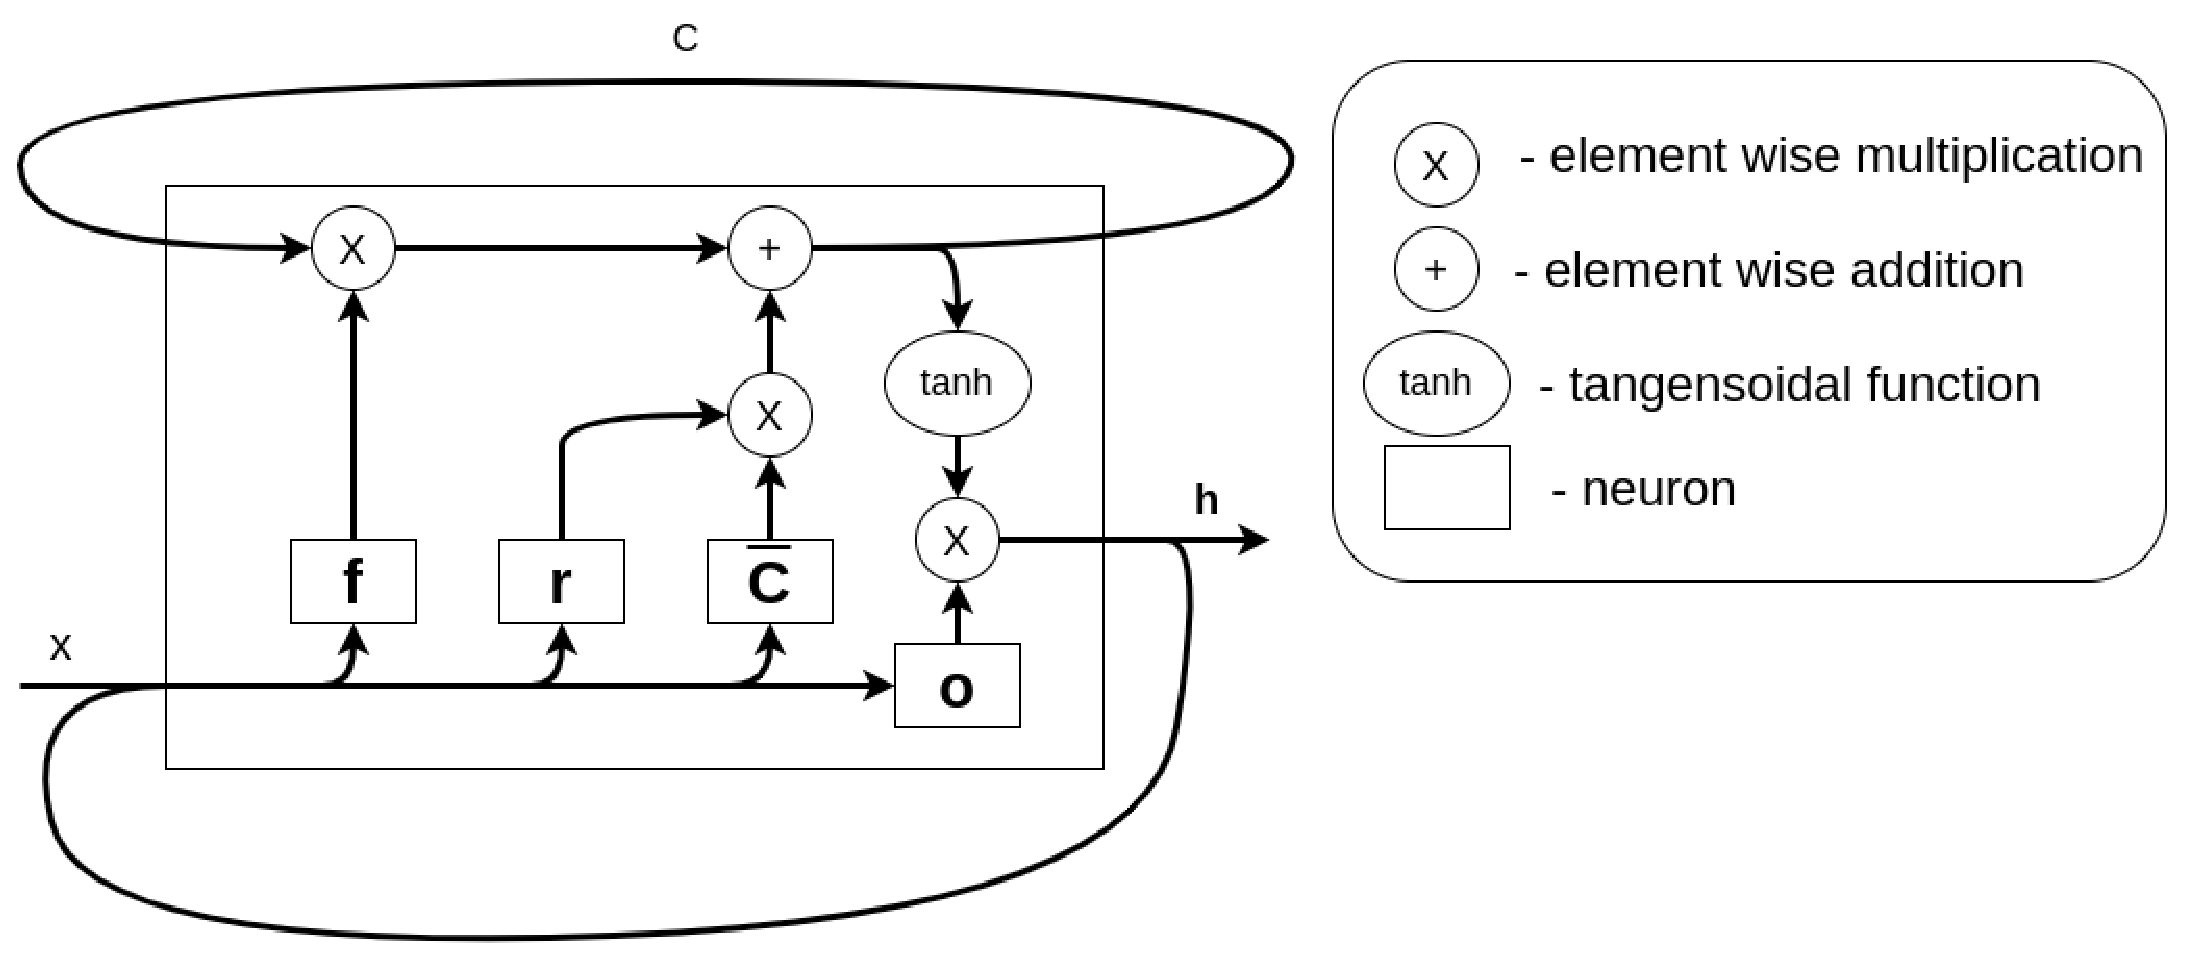
\includegraphics[width=10cm]{figures/lstm}
\caption{LSTM layer}
\label{fig:lstm}
\end{figure}
Single LSTM neuron consists of 4 basic neurons and two non neuron operations:
\begin{itemize}
\item $x'(t)=[x(t)|y(t-1)]$
\item $o_t=\sigma (W_o\cdot x'_t+b_o)$
\item $r_t=\sigma (W_r\cdot x'_t+b_r)$
\item $f_t=\sigma (W_f\cdot x'_t+b_f)$
\item $\bar{C}_t=\tanh (W_c\cdot x'_t+b_c)$
\item $C_t=f_t\circ C_{t-1}+r_t\circ \bar{C}_t$
\item $y_t=o_t\circ \tanh (C_t)$
\end{itemize}
With $W$ and $b$ being weights and biases for each basic neuron, $x$ input, $y$ output and
$C$ long term memory. As it can be seen $o_t$ is a equivalent of SRU and is moderated by
long term memory before propagating as output. Temporary value of long term memory based
only on current output $\bar{C}_t$ is calculated and then with help of neurons $r$ and $f$
is transformed into its final value.
Neuron $r$ is called remembering gate and influences to what degree temporary long term
memory from given cycle effects its final value while $f$ is forgetting gate and
decides influence of long term memory from last cycle on current one.
Thanks to such implementation model can learn to detect long term regularities as well
as short term ones.

%--------------------------------------------------------------------------------------------------
\subsection{Overfitting}  
Overfitting takes place when estimator function is adjusted to training data to such high
degree that it can no longer function as a general predictor.
For example if a network that is supposed to recognise cats will be trained on set that contains
only sphinxes it may be unable to classify other breeds as cats.
Overfitted networks provide very high quality results as long as input overlap with test set
otherwise quality of results drop sharply.
In case of satellite clocks predictor can overfit in regards to following parameters:
\begin{itemize}
\item clock type
\item location (orbit)
\item epoch
\end{itemize}
When selecting a solution a decision must be made on what level of generalisation model should
represent. Limiting predictions to same epochs that were used for training is in contradiction
with network main goal, predicting future biases. However as satellites use different models
of atomic clocks and are placed on different orbit attempts at generalisation for those
proprieties risk to high precision trade off.
Therefore a separate network will be used for each satellite that will be unable to generalize
its predictions to others.

%==================================================================================================
\section{Experiments}

%--------------------------------------------------------------------------------------------------
\subsection{Overview}
Experiments were divided in three phases:
\begin{enumerate}
\item In first phase a single satellite was selected and prediction with generic LSTM architecture
	was made. Then it was compared against polynomial regression as well as IGU rapid predictions.
	While achieving results better than polynomial regression would be considered acceptable at 
	this stage would be considered acceptable LSTM proved to be better than IGU example which
	was considered state of the art. Because of that a decision was made not to adjust network
	model at this stage, as was originaly intended, but move to next stage with a initial model.

\item In second phase network developed in first phase was tested on set of all active 
	satellites and compared agains IGU rapid prediction. At this phase comparition against 
	polynomial regression was dropped as achieving results worse than IGU was no longer 
	considered acceptable. In this phase for 5 of 31 satellites LSTM achieved better 
	results than IGU.

\item As second phase provided acceptable results only for a small group of satellites 
	an alternative arhcitectures were tested, more details about them will be writen in 
	dedicated section. In this phase results better than IGU were achieved 
	for 13 od 30 satellites.
\item Final phase was dedicated to tuning learning metaparameters and it results are described
	in more details in section dedicated to experiments.

\end{enumerate}
\makesubmdate

%==================================================================================================
\begin{thebibliography}{000}
% References should be listed in alphabetical order.

% For books, research reports and proceedings
\bibitem{B}
Author(s):
\newblock{Title of book.}
\newblock{Edition (if other than first). Publisher's name, place and year of publication (For books, research reports and proceedings).}

% Example
\bibitem{HoTu96}
R.~Horst and H.~Tuy:
\newblock{Global Optimization.}
\newblock{Springer--Verlag, Berlin 1996.}

% For journal article
\bibitem{P}
Author(s):
\newblock{Title of paper.}
\newblock{Title of the journal (abbreviated in accordance with Math. Reviews), volume, year of publication in brackets, inclusive pagination (For journal article).}

% Example
\bibitem{No85}
M.~Nov\'{a}k:
\newblock{A note on the algorithms for determining the model structure.}
\newblock{Kybernetika {\mi 21} (1985), 164--178.}

% For a paper in a bound collection
\bibitem{PC}
Author(s):
\newblock{Title of paper.}
\newblock{In: Title of collection, editor name(s) (in brackets), publisher's name, place and year of publication, inclusive pagination (For a paper in a bound collection).}

% Example
\bibitem{Pe81}
V.~Peterka:
\newblock{Bayesian system identification.}
\newblock{In: Trends and Progress in System Identification (P.~Eykhoff, ed.), Pergamon Press, Oxford 1981, pp. 239--304.}

\end{thebibliography}

\makecontacts

\end{document}


